
\section{Results}

\begin{frame}{Results}
  
  Revisiting the model
  $$\begin{cases}
    \begin{array}{rl}
      dM\hspace{-.8em}&=[aMC - \frac{gM(t-\tau)}{1-C(t-\tau)} + \gamma M (1-M-C)]dt+\beta M(1-M)dW,\\
      dC\hspace{-.8em}&=[rC(1-M-C) - dC - aMC]dt.\\
    \end{array}
    \end{cases}$$\\
  We are interested in the effects of:
  \begin{itemize}
  \item $\theta$ (the initial condition)\\
  \item $\beta$\\
  \item $\tau$\\
  \item $g$\\
  \end{itemize}
  
  

\end{frame}

\begin{frame}{Theta}
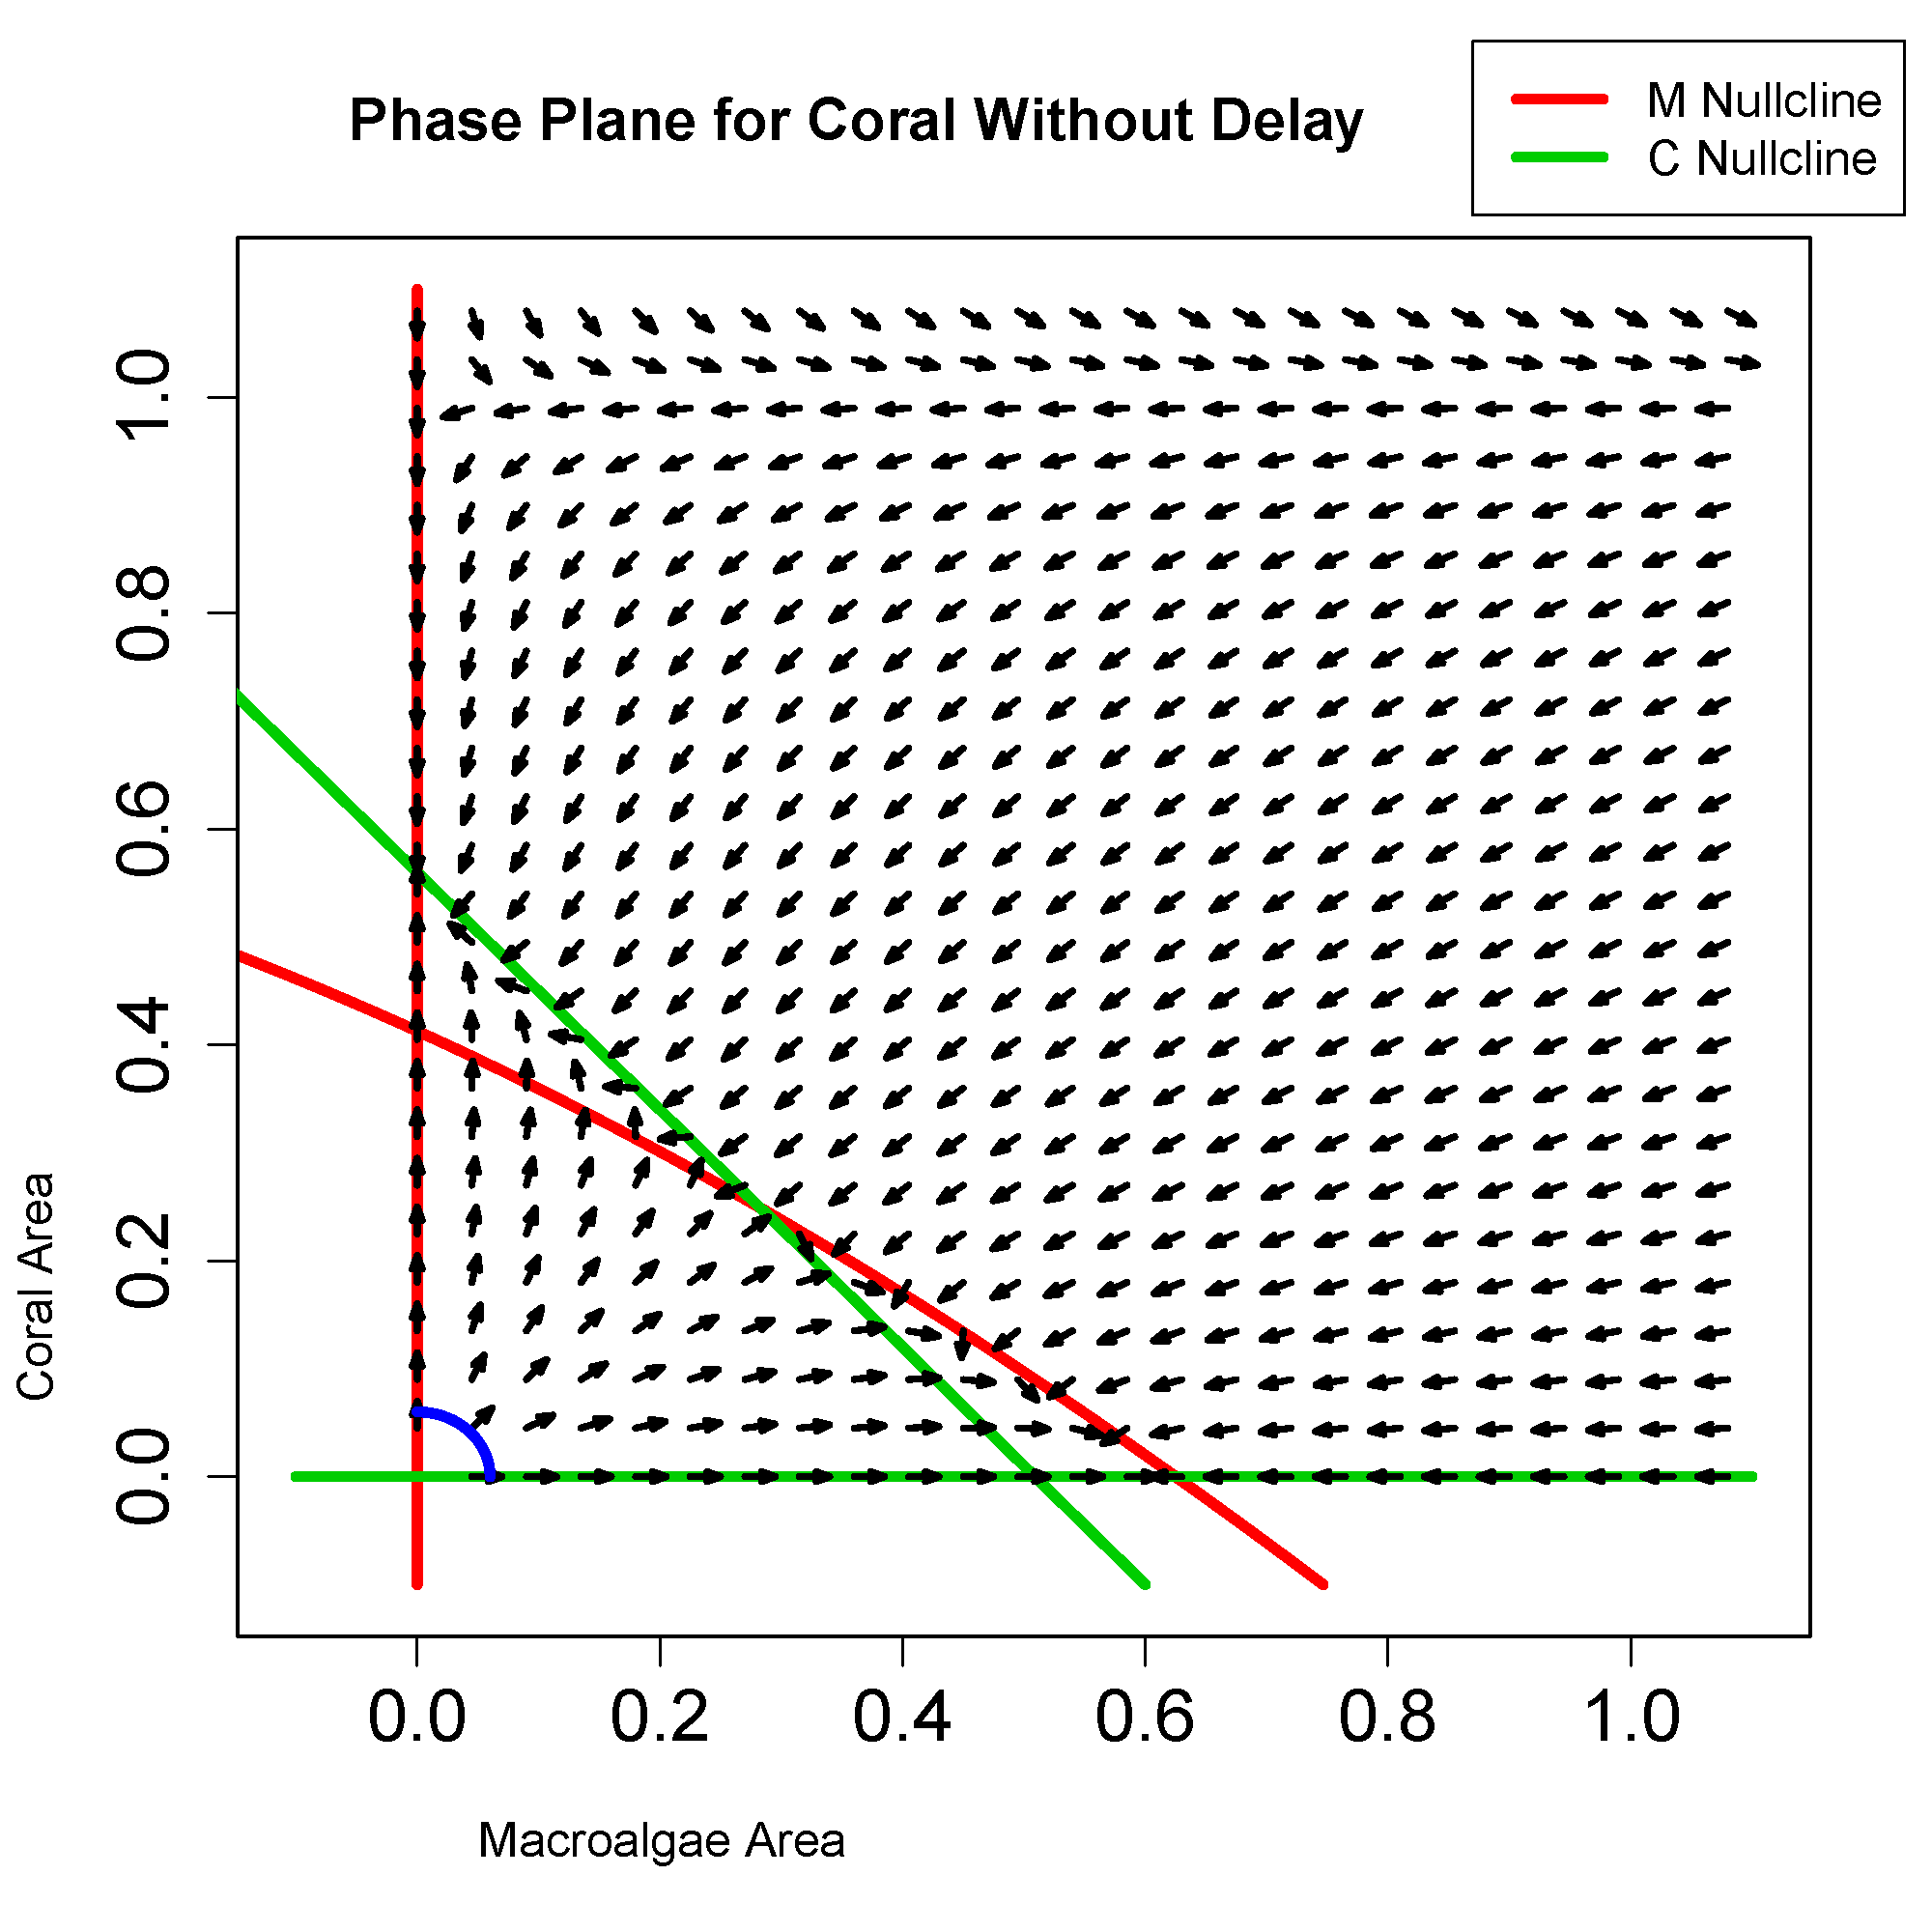
\includegraphics[scale=.325]{nullclinesarc.png}

\end{frame}

\begin{frame}{The Simulation}
We sampled the following values:
\begin{itemize}
\item $\theta$ = $\frac{\pi}{80}$ to $\frac{39\pi}{80}$ by $\frac{\pi}{80}$\\
\item $\beta$ = 0 to 1 by 0.05\\
\item $\tau$ = 0.5 to 1 by 0.05\\
\item $g$ = 0.2 to 0.8 by 0.1\\
\end{itemize}
\end{frame}

% %\begin{frame}\frametitle{At First Glance}
% %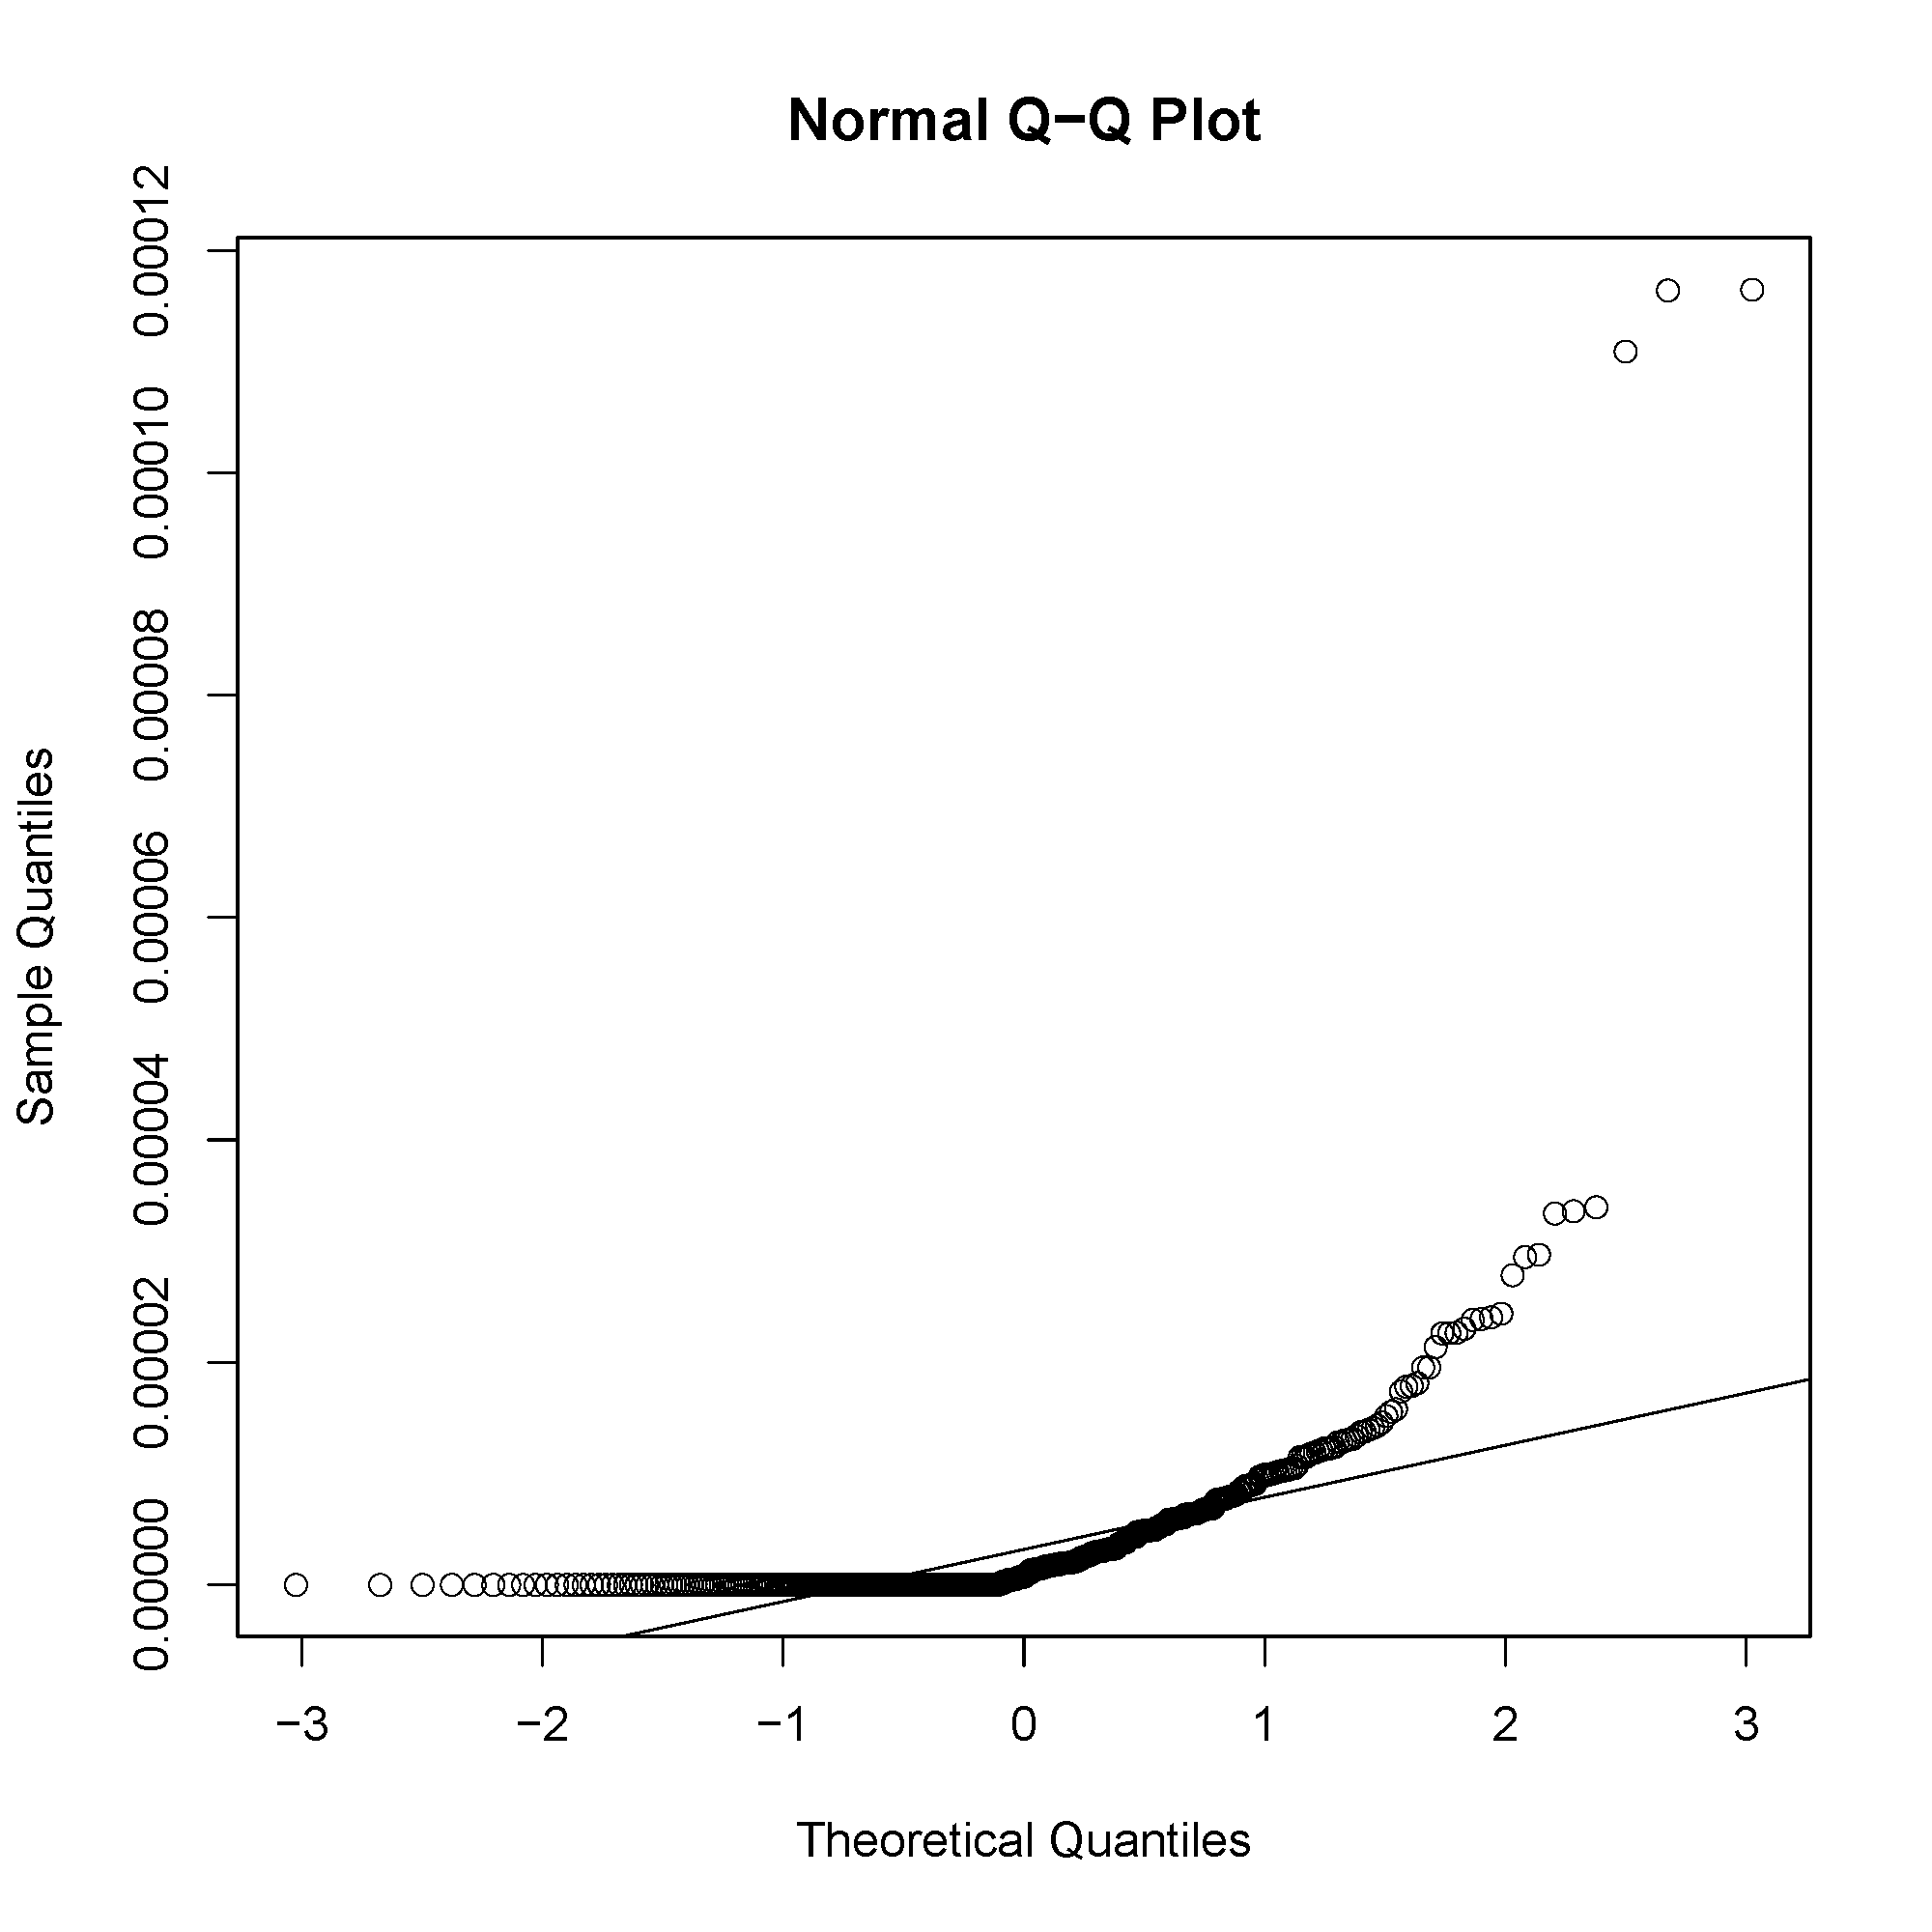
\includegraphics[scale=.325]{qqplot_lgcoral.png}
% %\end{frame}

\begin{frame}
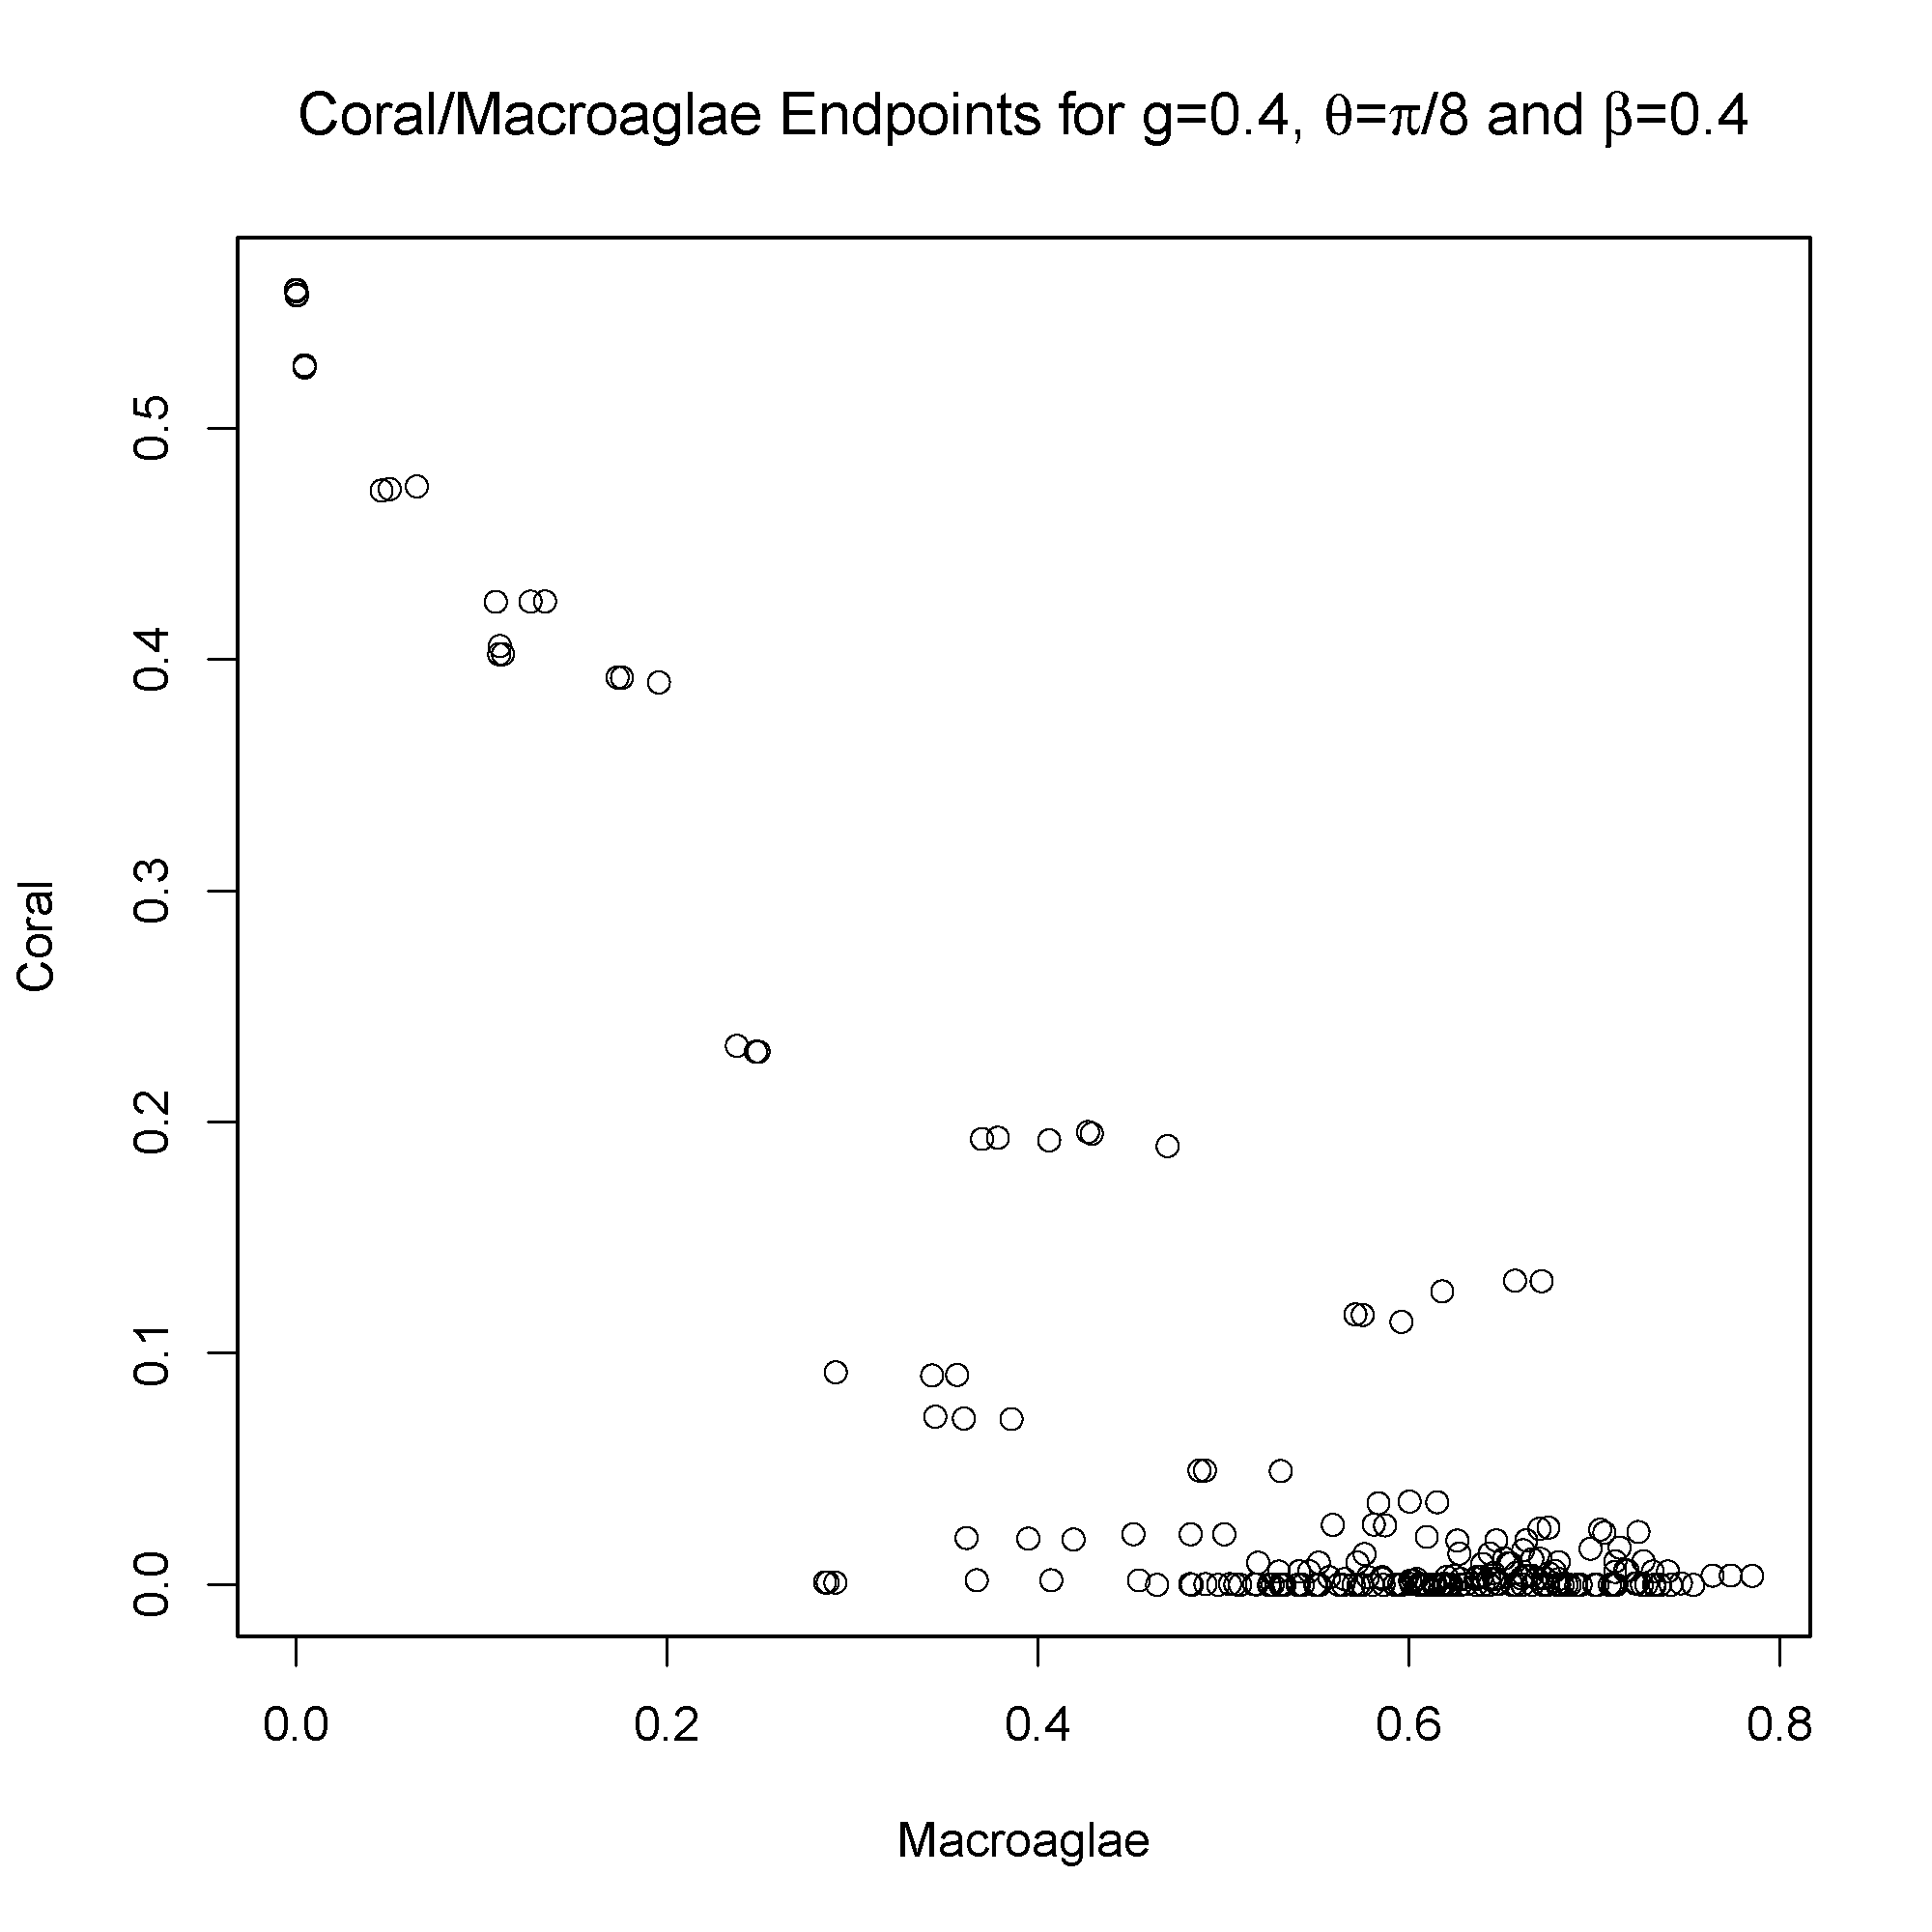
\includegraphics[scale=.325]{scatter_lgcoral_gpt4_betapt4_theta10.png}
\end{frame}

\begin{frame}{Initial Conditions}
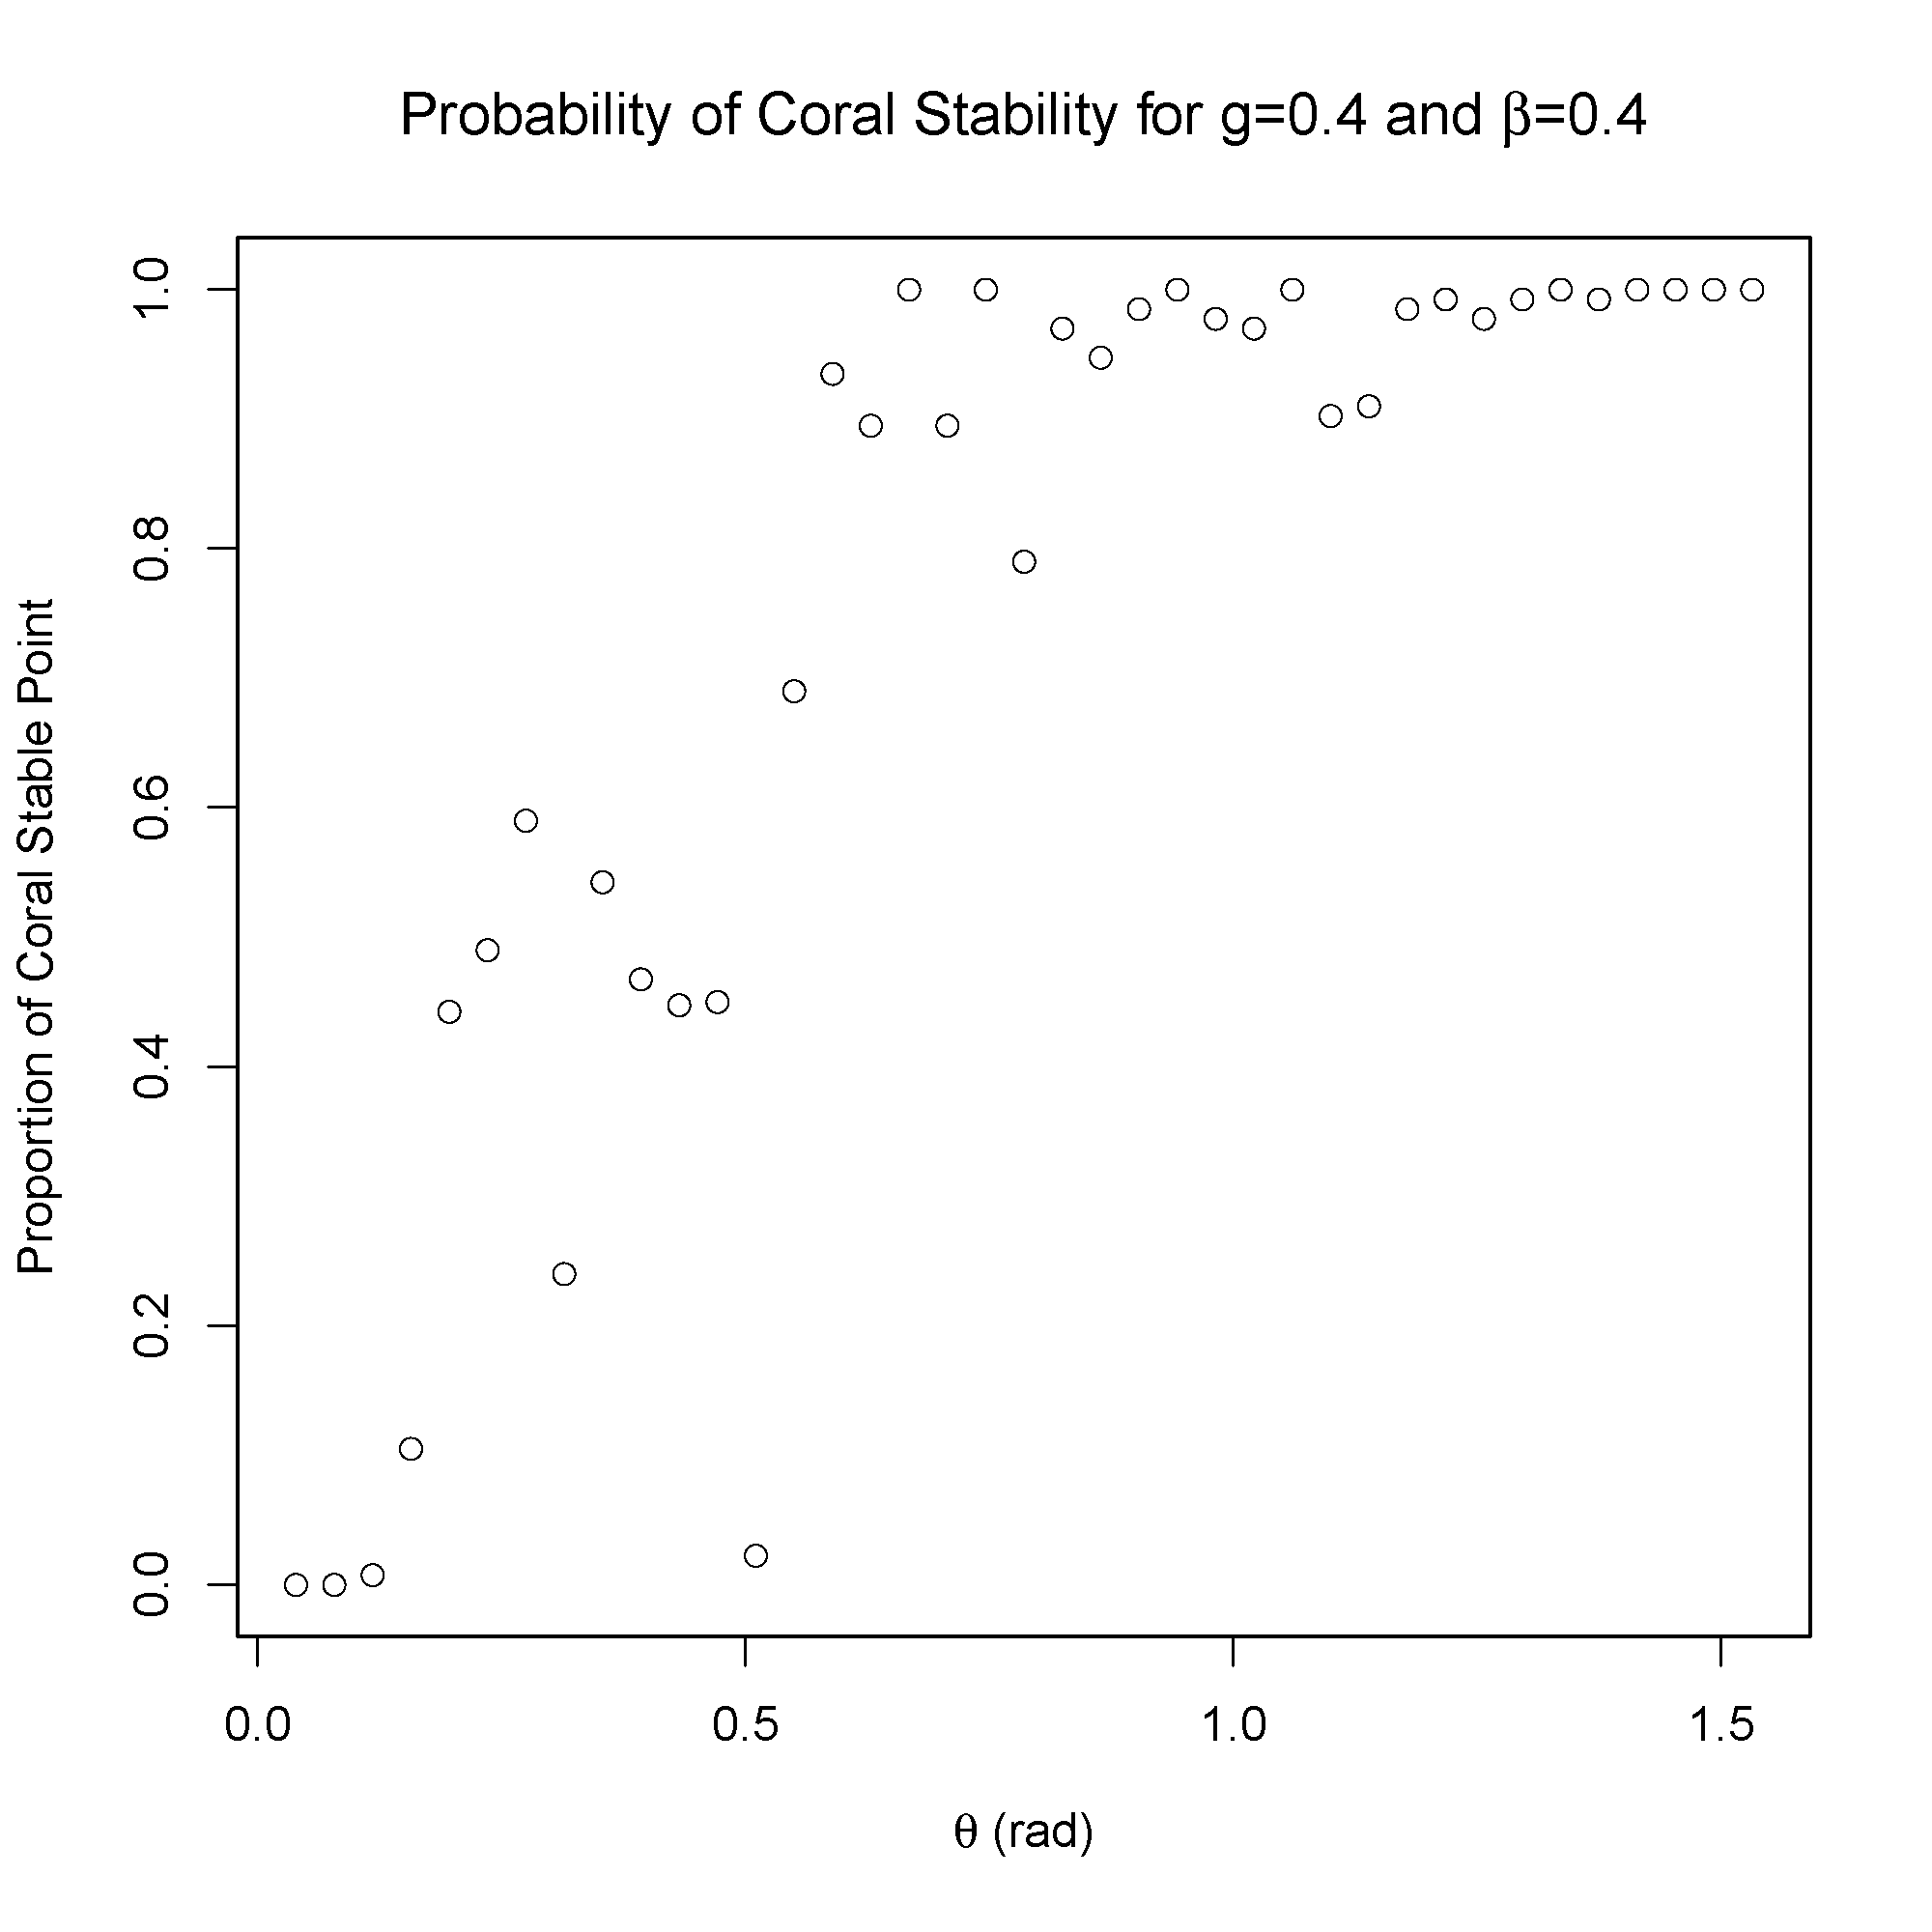
\includegraphics[scale=.325]{scatter_gpt4_betapt4.png}
\end{frame}

\begin{frame}{The Three Models}
Based on the plot, we will try the following three models
\begin{itemize}
\item Binomial Logit\\
Fits the model $logit(p)=a+b\theta$ where $logit(p)=log(\frac{p}{1-p})$\\
\item Poisson Log\\
Fits the model $log(n)=a+b\theta$\\
\item Ordinary Least Squares (OLS)\\
Fits the model $p=a+b\theta$\\
\end{itemize}
\end{frame}




\begin{frame}\frametitle{The Binomial Logit Model}
{\fontsize{8}{3} \color{RBlue} \verbatiminput{theta_logit_summary.txt}}

Conducting a goodness of fit test: \\
$P(\chi^{2}_{1}>10485-2171)<0.0001$\\

\end{frame}

\begin{frame}\frametitle{The Poisson Log Model}
{\fontsize{8}{3} \color{RBlue} \verbatiminput{theta_log_summary.txt}}

Conducting a goodness of fit test: \\
$P(\chi^{2}_{1}>3714.9-1970.4)<0.0001$\\

\end{frame}

%\begin{frame}\frametitle{Problematic Poisson}
%From the summary statistics, there is a problem with overdispersion.\\
%\\
%$\frac{G^2}{df}\approx1$\\
%$\frac{2006.7}{37}\approx54.2$\\
%\\
%Therefore, we fit a negative binomial model.\\
%\end{frame}

%\begin{frame}\frametitle{The Negative Binomial}

%\end{frame}

\begin{frame}\frametitle{Problematic Poisson}
There may be a problem with the model.
In the data, there is an overabundance of zeros.
Therefore, we fit a zero-inflated Poisson model (ZIP).
{\fontsize{8}{3} \color{RBlue} \verbatiminput{theta_zeros.txt}}
\end{frame}

\begin{frame}\frametitle{The ZIP Model}
{\fontsize{8}{3} \color{RBlue} \verbatiminput{theta_log_zip_summary.txt}}
\end{frame}

\begin{frame}\frametitle{The OLS Model}
{\fontsize{8}{3} \color{RBlue} \verbatiminput{theta_ols_summary.txt}}

Conducting a goodness of fit test: \\
$P(\chi^{2}_{1}>4.5824-1.4317)\approx0.07589$\\

\end{frame}

\begin{frame}\frametitle{Comparing the Models}
Our three models are \\
\begin{itemize}
\item Binomial Logit $p=\frac{e^{-2.48378+6.01631\theta}}{1+e^{-2.48378+6.01631\theta}}$\\
\item Poisson Log $n=e^{4.89295+0.90423\theta}$\\
\item OLS $p=0.22856+0.64310\theta$\\
\end{itemize}
How do we determine which model is the most appropriate?\\
\end{frame}

\begin{frame}{Binomial Logit, Poisson Log, or OLS}
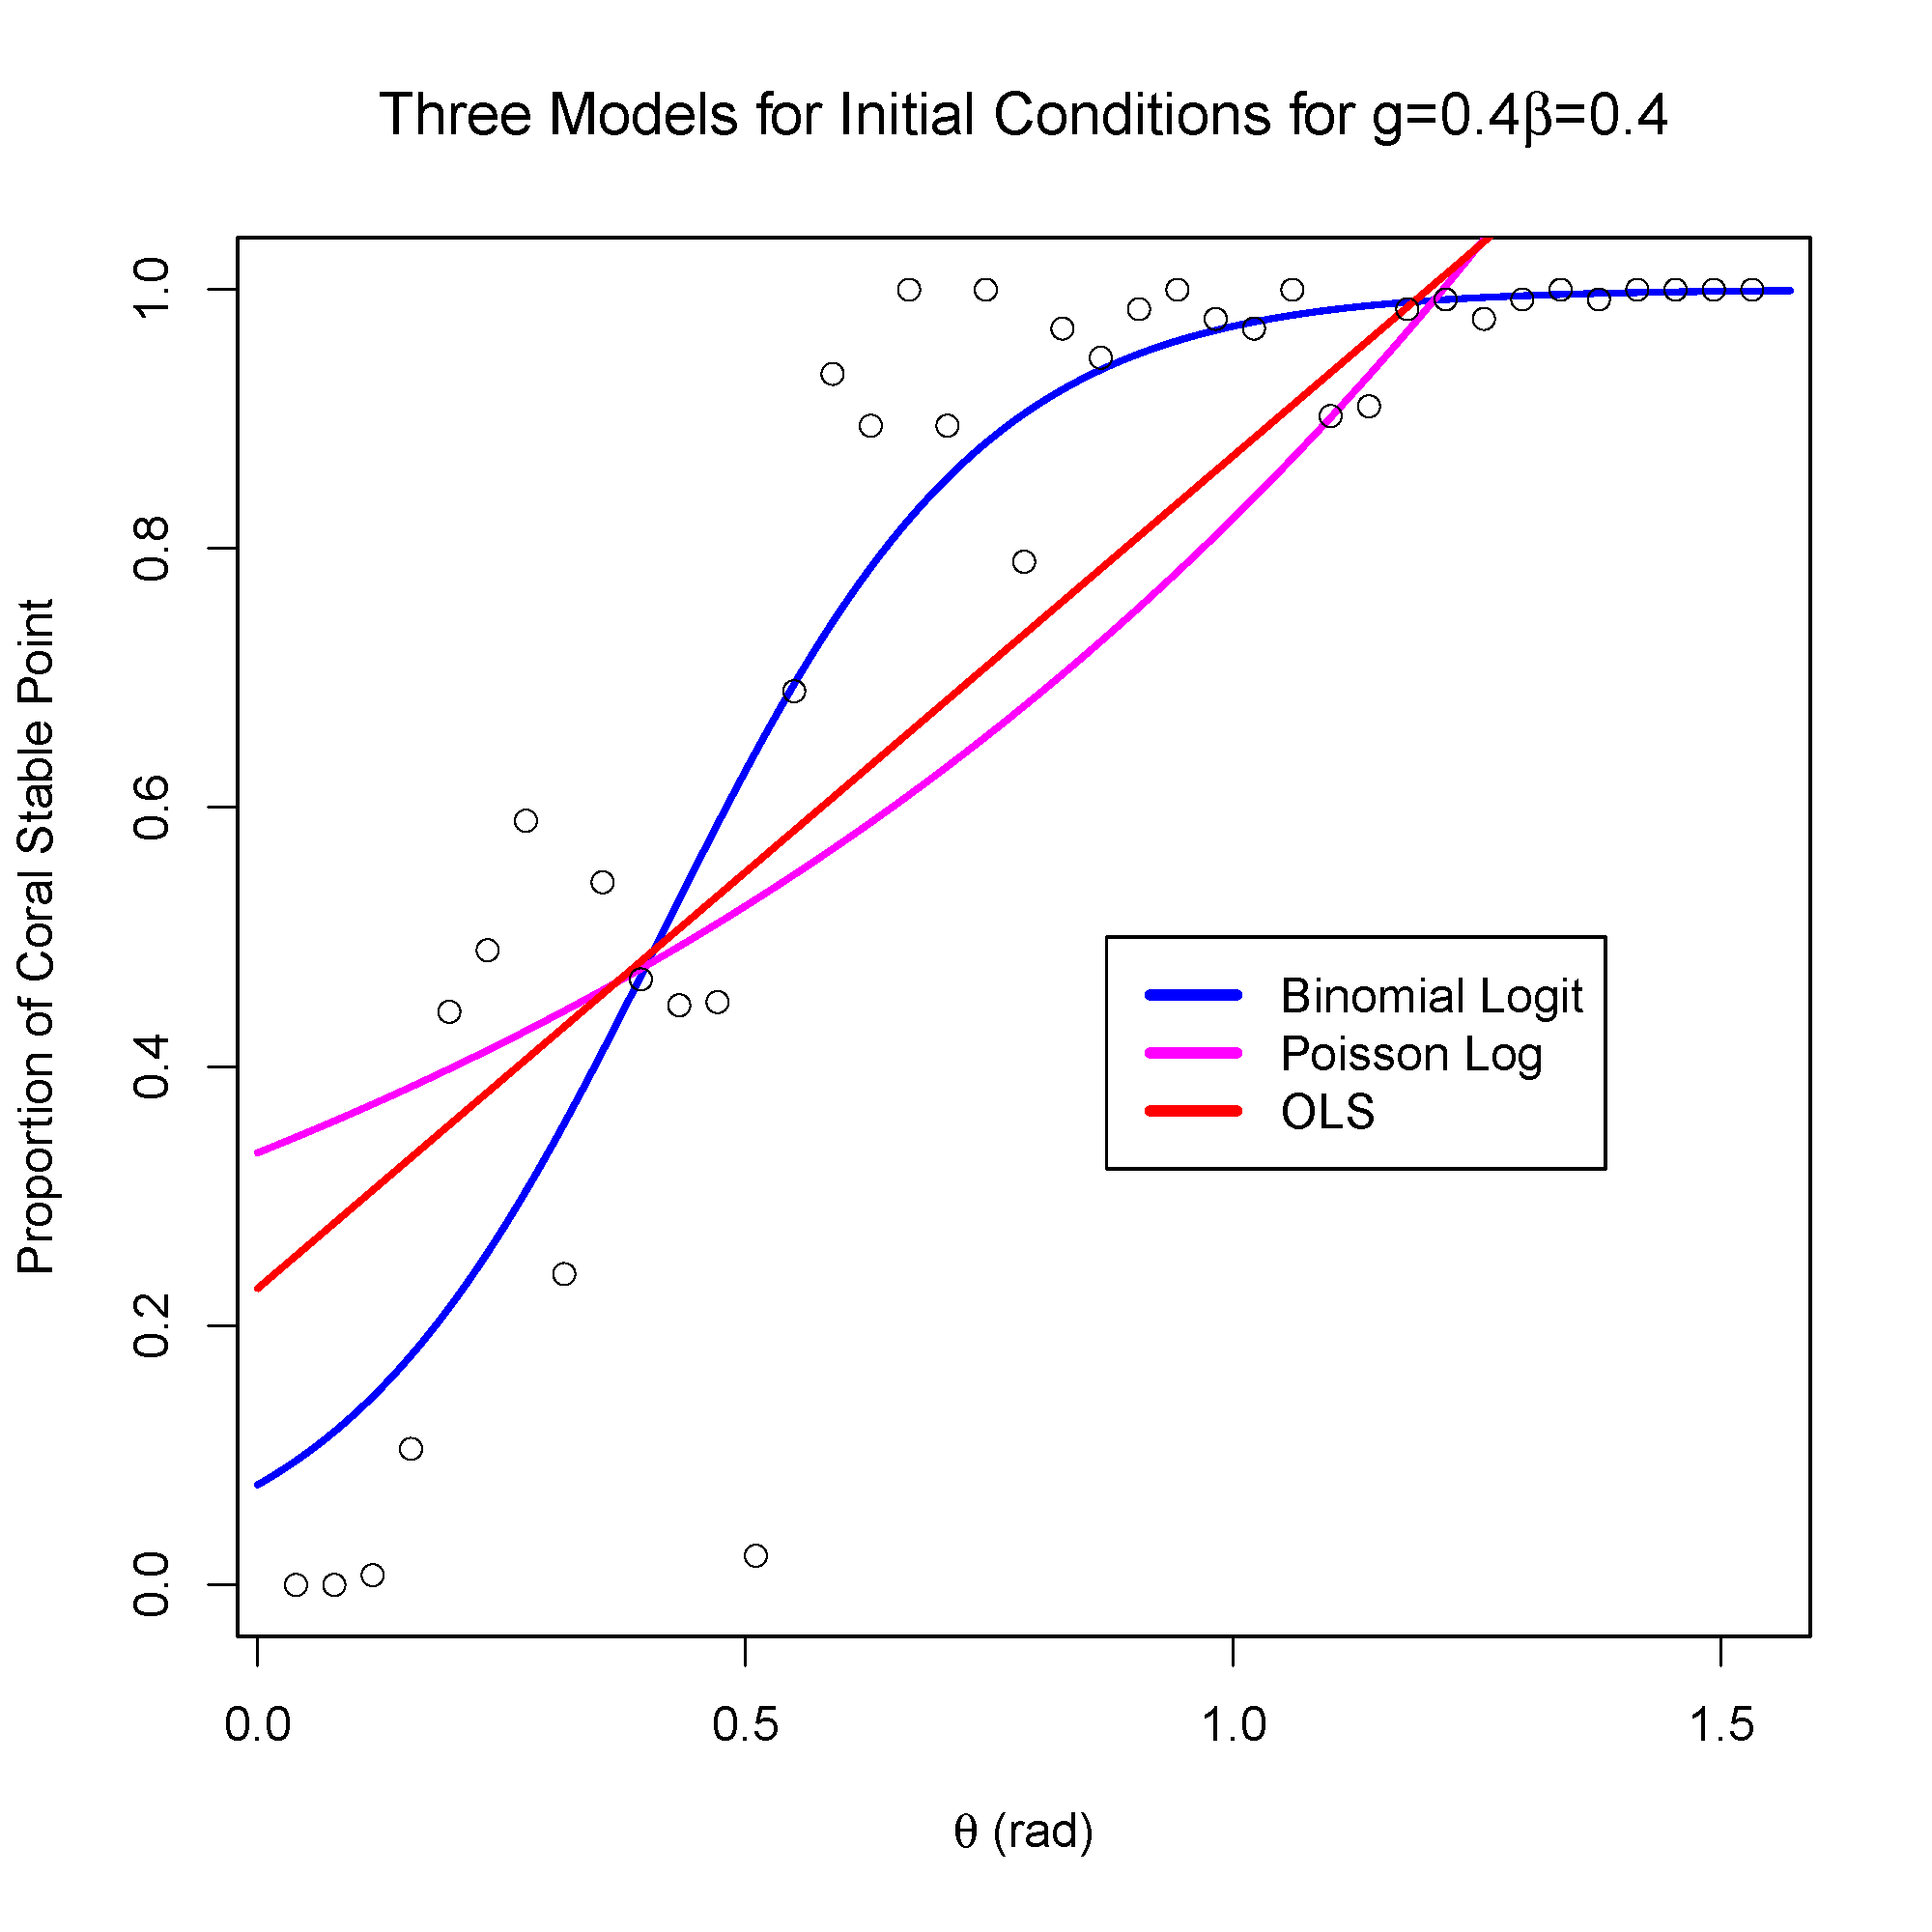
\includegraphics[scale=.325]{theta_threemodels.png}
\end{frame}

\begin{frame}\frametitle{The Whole Picture}
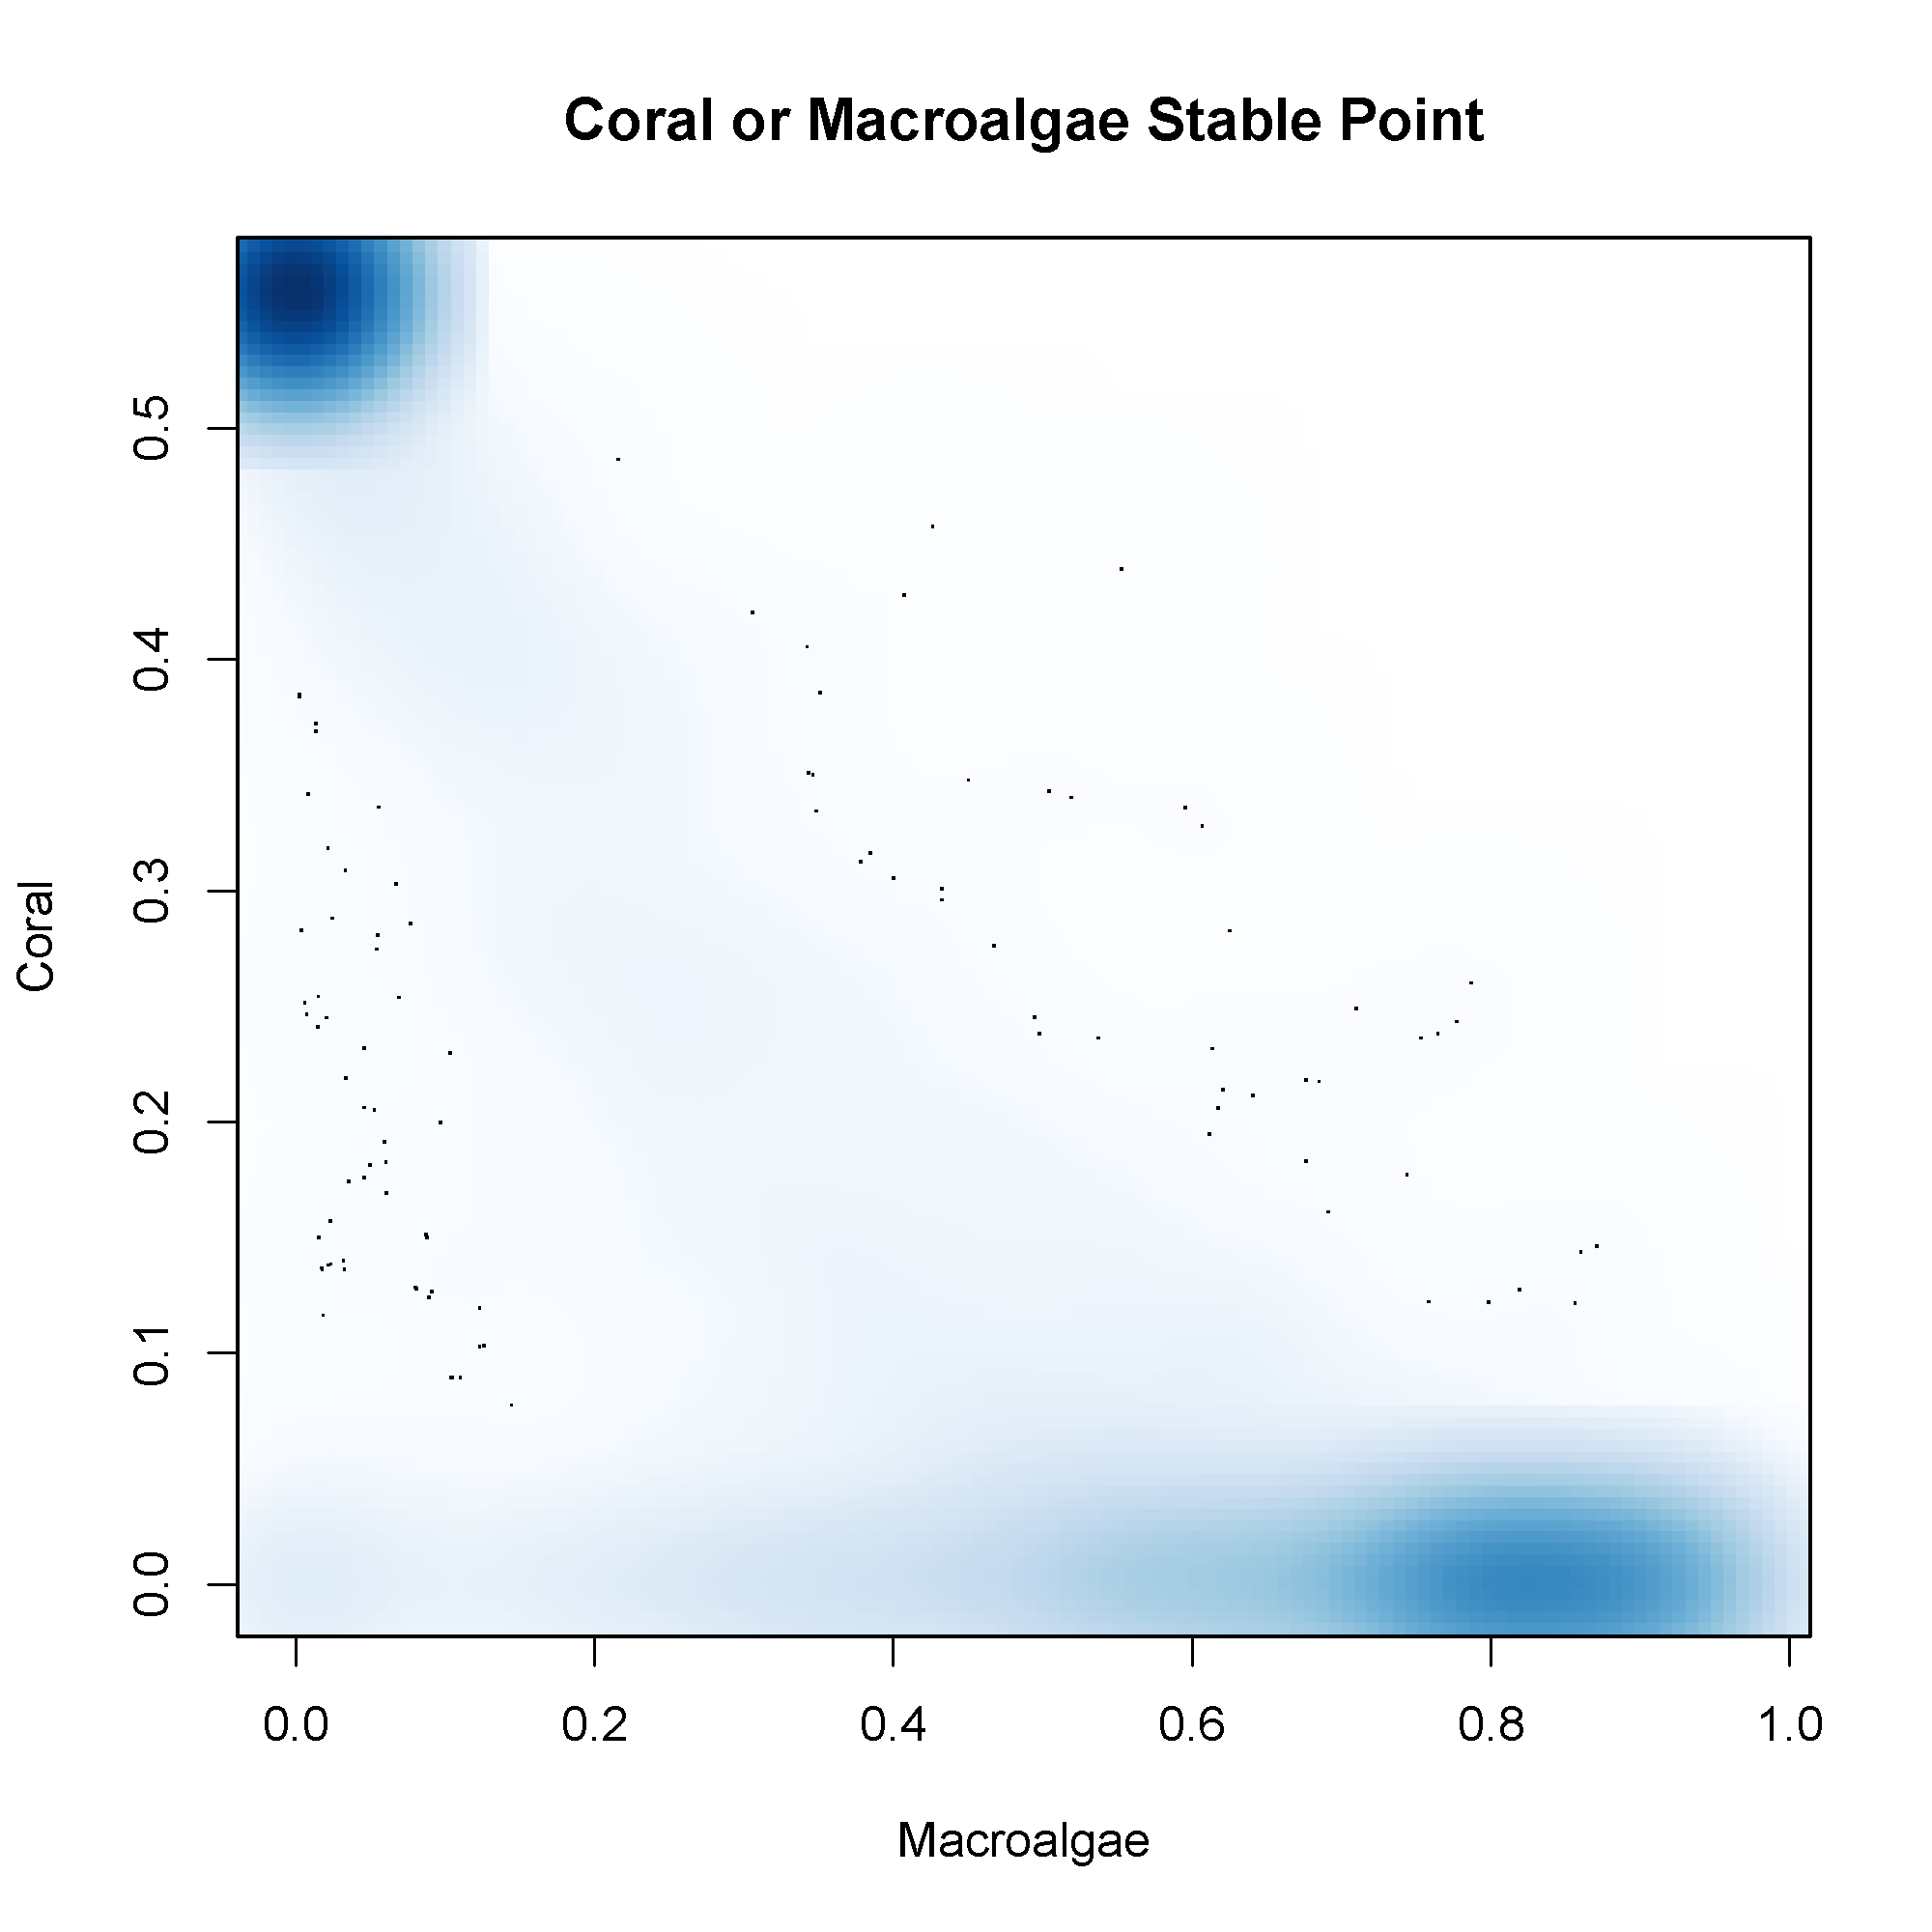
\includegraphics[scale=.325]{unifiedplot.png}
\end{frame}

\begin{frame}\frametitle{The Binomial Logit}
{\fontsize{8}{3} \color{RBlue} \verbatiminput{all_logit_summary.txt}}
\end{frame}

\begin{frame}\frametitle{Interpreting the Results}
Keeping theta and beta constant, an increase in g of:
\begin{itemize}
\item 0.01 has an odds ratio of coral survival of 3.21\\
\item 0.1 has an odds ratio of coral survival of 116413.1
\end{itemize}
\end{frame}

%%% Local Variables:
%%% mode: latex
%%% TeX-master: "Presentation2"
%%% End:
